\documentclass[11pt]{article}

\setlength{\textwidth}{6in}
\setlength{\oddsidemargin}{0.25in}
\setlength{\textheight}{9.0in}
\setlength{\topmargin}{-0.75in}

% common LaTeX macros
%
% Last modified: 03-02-2007
%

\usepackage{times}
%-------------------------
% the following magic makes the tt font in math mode be the same as the
% normal tt font (i.e., Courier)
%
\SetMathAlphabet{\mathtt}{normal}{OT1}{pcr}{n}{n}
\SetMathAlphabet{\mathtt}{bold}{OT1}{pcr}{bx}{n}
%-------------------------

\usepackage{amsmath}
\usepackage{amssymb} % for \pitchfork

\newcommand{\NOTE}[1]{%
  \par\leavevmode\noindent\textbf{[[ #1 ]]}\par\leavevmode\noindent}
\newcommand{\CUT}[1]{}
\newcommand{\SIDENOTE}[1]{%
  \marginpar{\tiny\raggedright{#1}}}

\newcommand{\appref}[1]{Appendix~\ref{#1}}
\newcommand{\chapref}[1]{Chapter~\ref{#1}}
\newcommand{\secref}[1]{Section~\ref{#1}}
\newcommand{\tblref}[1]{Table~\ref{#1}}
\newcommand{\figref}[1]{Figure~\ref{#1}}
\newcommand{\listingref}[1]{Listing~\ref{#1}}
\newcommand{\pref}[1]{{page~\pageref{#1}}}
\newcommand{\defref}[1]{Definition~\ref{#1}}
\newcommand{\ruleref}[1]{Rule~\ref{#1}}

\newcommand{\eg}{{\em e.g.}}
\newcommand{\cf}{{\em cf.}}
\newcommand{\ie}{{\em i.e.}}
\newcommand{\etc}{{\em etc.\/}}
\newcommand{\naive}{na\"{\i}ve}
\newcommand{\ala}{{\em \`{a} la\/}}
\newcommand{\etal}{{\em et al.\/}}
\newcommand{\role}{r\^{o}le}
\newcommand{\vs}{{\em vs.}}
\newcommand{\forte}{{fort\'{e}\/}}

%
% language names
\newcommand{\Cplusplus}{\mbox{C\hspace{-.05em}\raisebox{.4ex}{\tiny\bf ++}}}
\newcommand{\Cmm}{\mbox{C\hspace{-.05em}\raisebox{.4ex}{\small\textbf{{-}{-}}}}}
\newcommand{\csharp}{\textsc{C\#}}
\newcommand{\C}{\textsc{C}}
\newcommand{\Ckit}{\textsc{Ckit}}
\newcommand{\java}{\textsc{Java}}
\newcommand{\loom}{\textsc{Loom}}
\newcommand{\moby}{\textsc{Moby}}
\newcommand{\minimoby}{\textsc{MiniMoby}}
\newcommand{\micromoby}{\textsc{microMoby}}
\newcommand{\MOC}{\textsc{MOC}}
\newcommand{\ml}{\textsc{ML}}
\newcommand{\sml}{\textsc{SML}}
\newcommand{\smlnj}{\textsc{SML/NJ}}
\newcommand{\mlj}{\textsc{MLj}}
\newcommand{\cml}{\textsc{CML}}
\newcommand{\pml}{\textsc{PML}}
\newcommand{\ocaml}{\textsc{OCaml}}
\newcommand{\mlkk}{\textsc{ML2000}}
\newcommand{\haskell}{\textsc{Haskell}}
\newcommand{\mltwok}{\textsc{ML2000}}
\newcommand{\scala}{\textsc{Scala}}
\newcommand{\perl}{\textsc{Perl}}
\newcommand{\scheme}{\textsc{Scheme}}
\newcommand{\unix}{\textsc{Unix}}
\newcommand{\smalltalk}{\textsc{Smalltalk}}
\newcommand{\self}{\textsc{Self}}

%
% font commands
\providecommand{\bftt}[1]{{\ttfamily\bfseries{}#1}}
\providecommand{\ittt}[1]{{\ttfamily\itshape{}#1}}
\providecommand{\kw}[1]{\bftt{#1}}
\providecommand{\nt}[1]{{\rmfamily\itshape{#1}}}
\providecommand{\term}[1]{{\sffamily{#1}}}
%
% math-mode versions
\providecommand{\mkw}[1]{\ensuremath{\text{\kw{#1}}}}
\providecommand{\mnt}[1]{\ensuremath{\text{\nt{#1}}}}
\providecommand{\mterm}[1]{\ensuremath{\text{\term{#1}}}}

% braces (in math mode)
\newcommand{\LCB}{\mkw{\{}}
\newcommand{\RCB}{\mkw{\}}}

% underscore
\newcommand{\US}{\char`\_}

%%%%%
% Some common math notation
%

% double brackets
\newcommand{\LDB}{\ensuremath{[\mskip -3mu [}}
\newcommand{\RDB}{\ensuremath{]\mskip -3mu ]}}

\newcommand{\dom}{\ensuremath{\mathrm{dom}}}
\newcommand{\rng}{\ensuremath{\mathrm{rng}}}

% sets
\newcommand{\SET}[1]{\ensuremath{\{#1\}}}
\newcommand{\Fin}{\textrm{Fin}}     % finite power set
\newcommand{\DISJOINT}[2]{\ensuremath{#1 \pitchfork #2}}
\newcommand{\finsubset}{\mathrel{\stackrel{\textrm{fin}}{\subset}}}


% finite maps
\newcommand{\finmap}{\mathrel{\stackrel{\textrm{fin}}{\rightarrow}}}
\newcommand{\MAP}[2]{\SET{#1 \mapsto #2}}
\newcommand{\EXTEND}[2]{\ensuremath{#1{\pm}#2}}
\newcommand{\EXTENDone}[3]{\EXTEND{#1}{\MAP{#2}{#3}}}
\newcommand{\SUBST}[3]{\ensuremath{#1[#2\mapsto{}#3]}}
\newcommand{\SUBSTTWO}[5]{\ensuremath{#1[#2\mapsto{}#3,#4\mapsto{}#5]}}


% timestamp
\newcount\timeHH
\newcount\timeMM
\timeHH=\time
\divide\timeHH by 60
\timeMM=\time
\count255=\timeHH
\multiply\count255 by -60 \advance\timeMM by \count255
\newcommand{\timestamp}{%
  \today{} ---
  \ifnum\timeHH<10 0\fi\number\timeHH\,:\,\ifnum\timeMM<10 0\fi\number\timeMM}


\usepackage{graphicx}
\usepackage{listings}

\newenvironment{CCODE}
{\lstset{language=C}
\lstset{columns=flexible}
  \lstset{commentstyle=\textit}}

\title{VProc protocol}
\author{The Manticore Group}
\date{Draft of \today}

\begin{document}
\maketitle

\section{Overview}
This document describes the protocol for managing vprocs.

\section{Signaling and sleeping}\label{sec:signaling-and-sleeping}
This section presents the signaling and sleeping protocol used by vprocs.

\paragraph{Signals}
A signal is a fiber paired with fiber-local storage.
To handle a signal, a vproc initializes the fiber-local storage and runs the fiber to completion.

\paragraph{Landing pad}
The \emph{landing pad} is a lock-free linked list of incoming signals.
Each vproc owns a landing pad, and has access to all the other remote landing pads.
The landing pad supports two operations.
\begin{enumerate}
  \item Push a message on a remote landing pad.
  \item Pop all messages from the local landing pad.
\end{enumerate}

\paragraph{Sleeping}
When there is nothing to do, a vproc enters a temporary sleeping state, which lasts until either a
signal arrives on the vproc's landing pad or a global garbage collection is initiated by some other
vproc.
We avoid busy waiting by waiting on a condition variable provided by the Pthreads
library.
Unfortunately, the fact that the landing pad is a lock-free data structure causes
a problem:
signals might arrive after the vproc has checked the landing pad but before the vproc has
begun waiting on the condition variable.
Thus, there is a potential race condition that would allow the vproc to wait indefinitely,
even when work becomes available.
Our protocols must address this race condition by using some additional
synchronization.

\paragraph{VProc operations}
Below are the operations that the vproc protocol must provide.
\begin{itemize}
  \item Place a signal on the landing pad of a remote vproc. This operation also forces the
    vproc to stop and handle the incoming signal. The vproc is guaranteed to handle the signal
    within a constant number of computational steps.
    \footnote{Note that this operation has undefined behavior when applied to the host vproc.}
    \begin{CCODE}
      \begin{lstlisting}
      void VProcSendSignal (VProc_t *vp, Fiber_t *k, Value_t *fls);
    \end{lstlisting}
    \end{CCODE}
  \item Receive signals from the host vproc's landing pad. 
    \footnote{Note that this operation has undefined behavior when applied to a remote vproc.}
    \begin{CCODE}
    \begin{lstlisting}
      Value_t VProcRecvSignal (VProc_t *host);
        \end{lstlisting}
    \end{CCODE}
  \item Put the host vproc to sleep until its landing pad becomes nonempty.
    \footnote{Note that this operation has undefined behavior when applied to a remote vproc.}
    \begin{CCODE}
    \begin{lstlisting}
      void VProcSleep (VProc_t *host);
        \end{lstlisting}
    \end{CCODE}
\end{itemize}

We choose to minimize the synchronization overhead of VProcSendSignal even at the expense of
increasing the overhead of VProcSleep.
The rationale is that, in the common case, the VProcSleep operation affects idle vprocs, whereas
the VProcSendSignal function affects working vprocs.

\paragraph{VProc components}
The vproc structure (\figref{fig:vproc-structure}) contains a few components that are relevant to this discussion.
\begin{itemize}
\item ldgPad - The landing pad.
\item lock - Mutex lock provided by the OS that protects vproc state.
\item cond - Condition variable provided by the OS that we use to put the vproc to sleep.
\item sleeping - True, when the vproc is sleeping.\footnote{It is only necessary for protocol 1.}
\item limPtr - Heap-limit pointer. By setting this value to zero, we can force
  interrupt the vproc while it is running, and thus can force the vproc to receive any pending high-priority
  signals. We use the limit pointer to implement the VProcSendSignal operation.
\end{itemize}

\begin{figure}
\begin{center}
\begin{CCODE}
\begin{lstlisting}
typedef struct struct_vproc VProc_t;
struct struct_vproc {
    ...
    Value_t       ldgPad;
    Mutex_t	  lock;
    Cond_t	  wait;
    bool          sleeping;
    Value_t       limPtr;
    ...
};
\end{lstlisting}
\end{CCODE}
\end{center}
\caption{The VProc structure.}\label{fig:vproc-structure}
\end{figure}

\paragraph{Landing pad representation}
The landing pad is represented by either one of the values below.
\begin{itemize}
\item Empty queue item.
\begin{CCODE}
\begin{lstlisting}
EMPTY
\end{lstlisting}
\end{CCODE}
\item A queue item consists of a fiber k and its fiber-local storage fls and the next queue item. We create
  queue items using the following constructor.
\begin{CCODE}
\begin{lstlisting}
MkQueueItem(k, fls, item)
    \end{lstlisting}
    \end{CCODE}
\end{itemize}

\paragraph{Memory consistency model}
We support PRAM consistency, which means the following.
All processes see their own writes in the order they were issued from the process.
Different processes, however, can see writes in different order.

\paragraph{OS support}
We use mutex locks, condition variables and barriers provided by the OS.
\begin{itemize}
  \item Initialize the mutex lock.
    \begin{CCODE}
      \begin{lstlisting}
        void MutexInit (Mutex_t *lock);
      \end{lstlisting}
    \end{CCODE}
  \item Acquire the mutex lock.
    \begin{CCODE}
      \begin{lstlisting}
        void MutexLock (Mutex_t *lock);
      \end{lstlisting}
    \end{CCODE}
  \item Release the mutex lock.
    \begin{CCODE}
      \begin{lstlisting}
        void MutexUnock (Mutex_t *lock);
      \end{lstlisting}
    \end{CCODE}
  \item Initialize the condition variable.
    \begin{CCODE}
      \begin{lstlisting}
        void CondInit (Cond_t *cond);
      \end{lstlisting}
    \end{CCODE}
  \item Wait on the condition variable.
    \begin{CCODE}
      \begin{lstlisting}
        void CondWait (Cond_t *wait, Mutex_t *lock);
      \end{lstlisting}
    \end{CCODE}
  \item Signal the condition variable.
    \begin{CCODE}
      \begin{lstlisting}
        void CondSignal (Cond_t *wait);
      \end{lstlisting}
    \end{CCODE}
  \item Initialize the barrier. 
    \begin{CCODE}
      \begin{lstlisting}
        void BarrierInit (Barrier_t *barrier, int nProcs);
      \end{lstlisting}
    \end{CCODE}
  \item Wait on the barrier.
    \begin{CCODE}
      \begin{lstlisting}
        void BarrierWait (Barrier_t *barrier);
      \end{lstlisting}
    \end{CCODE}
\end{itemize}

\paragraph{VProcSendSignal}
The VProcSendSignal operation (\figref{fig:protocol1-send}) consists of two phases: 
\begin{enumerate}
  \item The operation repeatedly attempts to place a signal on the landing pad (lines 4-8).
  \item Once the signal has successfully entered the landing pad (line 10), the operation proceeds
    to notify the vproc of the signal, first by zeroing out the limit pointer (line 10), and then
    by signaling the vproc to wake it from sleeping (lines 11-12).
\end{enumerate}

\begin{figure}
\begin{CCODE}
\lstset{numbers=left}
\begin{lstlisting}
void VProcSendSignal (VProc_t *self, VProc_t *vp, Value_t fls, Value_t k)
{
    while (true) {
      Value_t landingPadOrig = vp->landingPad;
      Value_t landingPadNew = MkQueueItem(self, fls, k, landingPadOrig);
      Value_t x = CompareAndSwapValue(&(vp->landingPad), landingPadOrig, landingPadNew);
      if (ValueToPtr(x) != ValueToPtr(landingPadOrig)) {
	  continue;
      } else {
        vp->limPtr = PtrToValue(0);
	if (vp->sleeping == M_TRUE)
	    CondSignal(&(vp->wait));
	return;
      }
    }
}
\end{lstlisting}
\end{CCODE}
\caption{Protocol 1 VProcSendSignal operation.}\label{fig:protocol1-send}
\end{figure}

\paragraph{VProcRecvSignal}
The VProcRecvSignal operation (\figref{fig:protocol1-recv}) attempts to retrieve all pending signals from the
landing pad at once.
If the attempt fails or the landing pad is empty, VProcRecvSignal simply returns an empty list (lines 5 and 10).
If successful, VProcRecvSignal sets the landing pad to empty and returns the list of pending signals (line 8).

\begin{figure}
\begin{CCODE}
\lstset{numbers=left}
\begin{lstlisting}
Value_t VProcRecvSignal (VProc_t *host)
{
  Value_t ldgPadOrig = host->ldgPad;
  if (ValueToPtr(ldgPadOrig) == EMPTY)
    return PtrToValue(M_NIL);
  Value_t x = CAS(&(host->ldgPad), ldgPadOrig, EMPTY);
  if (ValueToPtr(x) == ValueToPtr(ldgPadOrig))
    return PtrToValue(ldgPadOrig);
  else
    return PtrToValue(M_NIL);
}
\end{lstlisting}
\end{CCODE}

\caption{Protocol 1 VProcRecvSignal operation.}\label{fig:protocol1-recv}
\end{figure}

\paragraph{VProcSleep}
The VProcSleep operation (\figref{fig:protocol1-sleep}) puts the vproc to sleep by 
setting the sleeping flag and subsequently waiting until the landing
pad becomes nonempty.
Note that due to the PRAM memory consistency model, we must use atomic write instructions (lines 4 and 7)
to prevent a race condition.
If we did not use atomic writes, it would be possible for a vproc to see that its
landing pad is empty while a remote vproc sees that the sleeping flag is set to true.
The timeline in \figref{fig:memory-consistency} depicts such a situation.

\begin{figure}
\begin{center}
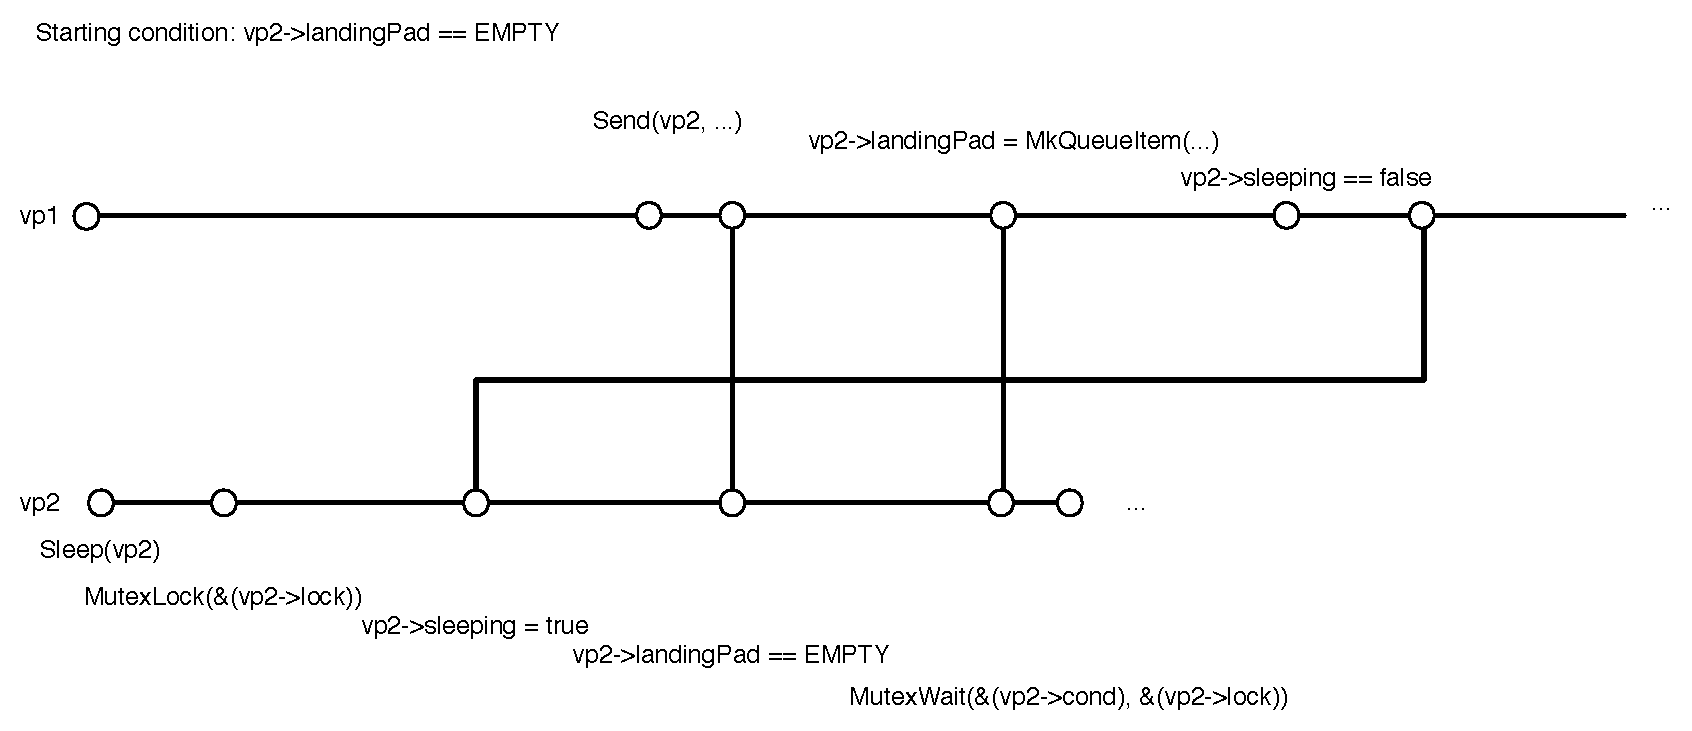
\includegraphics[scale=0.54]{pictures/vproc-protocol-memory-consistency}
\end{center}
\caption{Memory consistency issue.}\label{fig:memory-consistency}
\end{figure}

\paragraph{Correctness}
The correctness of this protocol is apparent from the following observation.
If, when the vproc tries to go to sleep, it sees that its landing pad is empty
(line 5 of \figref{fig:protocol1-sleep}), the other vprocs see that this vproc is sleeping.
Thus, it must be the case that all subsequent sends to that vproc are garanteed to
wake the vproc from its sleeping state (line 11 of \figref{fig:protocol1-send}).

\begin{figure}
\begin{CCODE}
\lstset{numbers=left}
\begin{lstlisting}
void VProcSleep (VProc_t *host)
{
  MutexLock(&(host->lock));
    AtomicWriteValue (&(vp->sleeping), M_TRUE);
    while (ValueToPtr(host->ldgPad) == EMPTY)
      CondWait(&(host->wait), &(host->lock));
    AtomicWriteValue (&(vp->sleeping), M_FALSE);
  MutexUnlock(&(host->lock));
}
    \end{lstlisting}
    \end{CCODE}

\caption{Protocol 1: VProcSleep operation.}\label{fig:protocol1-sleep}
\end{figure}

\section{Global garbage collection}\label{sec:global-gc}
Figure \ref{fig:global-gc-protocol} shows the protocol for starting a global garbage
collection.
The protocol assigns one vproc to be the leader.
The leader is responsible to initialize global state values and to notify other vprocs
that a collection is imminent.
Non-leader vprocs must participate in every collection, whether they are awake or asleep.

\paragraph{Global collector state}
Below is global state (shared by all vprocs) that we use in the protocol.
\begin{itemize}
  \item Mutex lock for the state.
    \begin{CCODE}
    \begin{lstlisting}
      static Mutex_t GCLock;
        \end{lstlisting}
    \end{CCODE}
  \item Condition variable for the lead vproc.
    \begin{CCODE}
    \begin{lstlisting}
      static Cond_t LeaderWait;
        \end{lstlisting}
    \end{CCODE}
  \item Condition variable for the non-lead vprocs.
    \begin{CCODE}
    \begin{lstlisting}
      static Cond_t FollowerWait;
        \end{lstlisting}
    \end{CCODE}
  \item Number of vprocs ready to begin a global collection.
    \begin{CCODE}
    \begin{lstlisting}
      static int NReadyForGC;
        \end{lstlisting}
    \end{CCODE}
  \item N-way barrier vprocs must pass before the collection can complete.
    \begin{CCODE}
    \begin{lstlisting}
      static Barrier_t GCBarrier;
        \end{lstlisting}
    \end{CCODE}
  \item True when a global collection is in progress.
    \begin{CCODE}
    \begin{lstlisting}
      static bool GlobalGCInProgress;
        \end{lstlisting}
    \end{CCODE}
\end{itemize}

\figref{fig:global-gc-protocol} shows the protocol for performing a global collection.
The protocol begins by assigning the vproc as lead or non-lead.
The lead vproc first initializes the state (lines 8-11) and then notifies the
other vprocs that a global collection is in progress (lines 21-23).
\footnote{The dummy fiber is a trivial fiber that we use to wake a vproc to participate
in a global collection.}
The leader then waits (lines 25-26) for the other vprocs to add their memory pages to the
from-space list (line 18).
Once all vprocs have passed this initialization phase (lines 3-19), the global collection
can begin (line 30).
The barrier (line 33) marks the point that the collection ends.

\begin{figure}
\begin{CCODE}
\lstset{numbers=left}
\begin{lstlisting}
void StartGlobalGC (VProc_t *self, Value_t **roots)
{
  bool leaderVProc;
  MutexLock(&GCLock);
    if (!GlobalGCInProgress) {
      leaderVProc = true;
      GlobalGCInProgress = true;
      NReadyForGC = 1;
      BarrierInit(&GCBarrier, NumVProcs);
      for (int i = 0; i < NumVProcs; i++)
        if (VProcs[i] != self)
          VProcSendSignal(VProcs[i], self->dummyCont, self->currentFLS);
    } else {
      leaderVProc = false;
      if (++NReadyForGC == NumVProcs)
         CondSignal(&LeaderWait);
      CondWait(&FollowerWait, &GCLock);
    }
  /* ... adding the vproc's pages to the from-space list ... */
  MutexUnlock(&GCLock);
  if (leaderVProc) {
    MutexLock(&GCLock);
      while (NReadyForGC < NumVProcs)
        CondWait(&LeaderWait, &GCLock);
      CondBroadcast(&FollowerWait);
    MutexUnlock(&GCLock);    
  }
  /* ... running the global garbage collector ... */
  if (leaderVProc) {
    /* reclaim from-space pages */
    GlobalGCInProgress = false;
  }
  BarrierWait(&GCBarrier);
}
    \end{lstlisting}
    \end{CCODE}
\caption{The global garbage collection protocol.}\label{fig:global-gc-protocol}
\end{figure}

\CUT{
\subsection{Protocol 2}\label{sec:protocol2}

\paragraph{Landing pad representation}
The landing pad is represented the same way as in protocol 1, except that it 
contains an additional state called SLEEPING.

\paragraph{VProcSendSignal}
The VProcSendSignal operation (\figref{fig:protocol2-send}) takes one of two based on the assumed
vproc state:
\begin{itemize}
\item \emph{The vproc is assumed awake (lines 6-11).} We attempt to push a signal on the remote vproc's landing pad (lines 6-7), and
if the push fails, we retry the operation (line 11).
\item \emph{The vproc is assumed sleeping (lines 13-21).} We obtain a mutex lock from the vproc, and test
whether it is still sleeping.
If so we place the signal on its landing pad and wake the vproc (lines 18-19), 
but otherwise release the lock and retry (lines 15-16).
\end{itemize}

\begin{figure}
\begin{CCODE}
\lstset{numbers=left}
\begin{lstlisting}
void VProcSendSignal (VProc_t *vp, Fiber_t *k, Value_t *fls)
{
  while (true) {
    QueueItem_t *ldgPadOrig = vp->ldgPad;
    if (ldgPadOrig != SLEEPING) {
      QueueItem_t *ldgPadNew = MkQueueItem(self, k, fls, ldgPadOrig);
      QueueItem_t *x = CAS(&(vp->ldgPad), ldgPadOrig, ldgPadNew);
      if (x == ldgPadOrig)
	return;
      else
	continue;
    } else {            /* (ldgPadOrig == SLEEPING) */
      MutexLock(&(vp->lock));
        if (vp->ldgPad != SLEEPING) {
          MutexUnlock(&(vp->lock));
          continue;
        }
        vp->ldgPad = MkQueueItem(k, fls, EMPTY);
        CondSignal(&(vp->wait));
      MutexUnlock(&(vp->lock));
      return;
    }
  }
}
\end{lstlisting}
\end{CCODE}
\caption{Protocol 2 VProcSendSignal operation.}\label{fig:protocol2-send}
\end{figure}

\paragraph{VPRocRecvSignal}
The VProcRecvSignal operation is identical to protocol 1, under the assumption that VProcRecvSignal is never called while
the vproc is in a sleeping state.

\paragraph{VProcSleep}
The VProcSleep operation (\figref{fig:protocol2-sleep}) acquires the lock
and then attempts to mark the state as sleeping (lines 3-4).
If this step succeeds, the vproc sleeps until a the landing pad becomes
nonempty (lines 5-6).
Once the vproc has woken up, it releases the lock (line 7).

\begin{figure}
\begin{CCODE}
\lstset{numbers=left}
\begin{lstlisting}
void VProcSleep (VProc_t *host)
{
  MutexLock(&(vp->lock));
    QueueItem_t *x = CAS(&(vp->ldgPad), EMPTY, SLEEPING);
    while (vp->ldgPad == SLEEPING)
      CondWait(&(vp->wait), &(vp->lock));
  MutexUnlock(&(vp->lock));
}
    \end{lstlisting}
    \end{CCODE}
\caption{Protocol 2: VProcSleep operation.}\label{fig:protocol2-sleep}
\end{figure}

\paragraph{Correctness}
The key observation for correctness is the following: if the vproc succeeds in 
entering a sleep state (line 4 \figref{fig:protocol2-sleep}), then exactly one other vproc executing a VProcSendSignal operation sees 
that this is the case (line 14 of \figref{fig:protocol2-send}).
Thus, if another vproc performs a VProcSendSignal operation, the destination vproc must always
leave its sleep state.

\subsection{Evaluation}\label{sec:evaluation}
Protocol 1 is conceptually simpler and requires fewer lines of code.
On the other hand, protocol 2 benefits from a potentially faster VProcSendSignal operation.
In the common case where the vproc is awake, a protocol-2 VProcSendSignal requires one less memory reference.
}

\end{document}  
